\documentclass[pdftex]{beamer} 
\usepackage{graphicx}
\usepackage{amsmath,amssymb,amsthm} 
\usepackage{pb-diagram}
\usepackage{ucs}
\usepackage[utf8x]{inputenc}
%\usepackage[russian]{babel}
\usepackage{epstopdf}
\usepackage{multicol}
\usepackage{cancel}

\usepackage{amsfonts}

%%%%%%%%%%%%%%%%%%%%%%%%%%%%%%%%%%%%%%%%%%%%%%%%%%%%%%%%%%%%%%%%%%%%%%%%%%%%%%%%%%%%%%%%%%%%%%%%%%%

%\newtheorem{theorem}{Theorem}
%% \newtheorem{acknowledgement}[theorem]{Acknowledgement}
%% \newtheorem{algorithm}[theorem]{Algorithm}
%% \newtheorem{axiom}[theorem]{Axiom}
%% \newtheorem{case}[theorem]{Case}
%% \newtheorem{claim}[theorem]{Claim}
%% \newtheorem{conclusion}[theorem]{Conclusion}
%% \newtheorem{condition}[theorem]{Condition}
%% \newtheorem{conjecture}[theorem]{Conjecture}
%% \newtheorem{mycorollary}[theorem]{Corollary}
%% \newtheorem{mycriterion}[theorem]{Criterion}
%% \newtheorem{mydefinition}[theorem]{Definition}
%% \newtheorem{myexample}[theorem]{Example}
%% \newtheorem{myexercise}[theorem]{Exercise}
\newtheorem{mylemma}[theorem]{Lemma}
%% \newtheorem{mynotation}[theorem]{Notation}
%% \newtheorem{myproblem}[theorem]{Problem}
%% \newtheorem{myproposition}[theorem]{Proposition}
%% \newtheorem{myremark}[theorem]{Remark}
%% \newtheorem{mysolution}[theorem]{Solution}
%% \newtheorem{mysummary}[theorem]{Summary}
%% \newenvironment{myproof}[1][Proof]{\textbf{#1.} }{\ \rule{0.5em}{0.5em}}


\newcommand{\go}{\stackrel{\circ }{\mathfrak{g}}}
\newcommand{\ao}{\stackrel{\circ }{\mathfrak{a}}}
\newcommand{\co}[1]{\stackrel{\circ }{#1}}
\newcommand{\pia}{\pi_{\mathfrak{a}}}
\newcommand{\piab}{\pi_{\mathfrak{a}_{\bot}}}
\newcommand{\gf}{\mathfrak{g}}
\newcommand{\gfh}{\hat{\mathfrak{g}}}
\newcommand{\af}{\mathfrak{a}}
\newcommand{\afh}{\hat{\mathfrak{a}}}
\newcommand{\bff}{\mathfrak{b}}
\newcommand{\afb}{\mathfrak{a}_{\bot}}
\newcommand{\hf}{\mathfrak{h}}
\newcommand{\hfg}{\hf_{\gf}}
\newcommand{\hfb}{\mathfrak{h}_{\bot}}
\newcommand{\pf}{\mathfrak{p}}
\newcommand{\aft}{\widetilde{\mathfrak{a}}}
\newcommand{\sfr}{\mathfrak{s}}
%\pagestyle{plain}

\theoremstyle{definition} \newtheorem{Def}{Definition}
\setbeamertemplate{caption}[empty]
\newcommand{\tr}{\hat\triangleright} \newcommand{\trc}{\triangleright}
\newcommand{\adk}{a^{\dagger}_{\kappa}} \newcommand{\ak}{a_{\kappa}}
\def\bF{\mbox{$\overline{\cal F}$}} \def\F{\mbox{$\cal F$}}

\usetheme{AnnArbor}
%\usetheme{Warsaw}

%% Модели Весса-Зумино-Новикова-Виттена и coset-модели -- это два важных
%% класса моделей двумерной конформной теории поля. Теория представления
%% аффинных алгебр Ли играет центральную роль при изучении таких моделей. 
%% Сингулярные векторы в модулях алгебры Ли аннигилируются повышающими
%% операторами. Набор этих векторов определяет структуры представления:
%% например, неприводимый модуль можно построить из модуля Верма путем
%% отщепления модулей Верма, соответствующих сингулярным векторам
%% (БГГ-резольвента). 
%% Мы рассмотрим структуру сингулярных элементов и свойства их разложения
%% по отношению к (аффинным) подалгебрам. Из этих свойств следуют
%% рекуррентные соотношения на коэффициенты ветвления и связь ветвления с
%% обобщенной резольвентой Бернштейна-Гельфанда-Гельфанда. Мы также
%% покажем, что разложение сингулярных элементов определяет структуру
%% модулей алгебры Вирасоро в coset-моделях конформной теории поля.
%% 
\title[On singular elements in CFT]{On singular elements in conformal field theory}
\author[A. Nazarov]{A. Nazarov and V.D. Lyakhovsky\\\small{arXiv:1007.0318, 1111.6787, 1204.1855}}%\\\small{По материалам кандидатской диссертации\\ см. также arXiv:1007.0318, 1102.1702, 1107.4681, 1111.6787, 1112.4354 \\ научный руководитель В. Д. Ляховский}}

\institute[SPbSU]{
  Department of High Energy and Elementary Particle Physics\\
  faculty of physics\\
  St Petersburg State University\\
  198904, St Petersburg, Russia\\
  e-mail: anton.nazarov@hep.phys.spbu.ru
}

\date[MQFT 2012] % (optional, should be abbreviation of conference name)
{27.09.2012}
\begin{document}
\maketitle

\section{Introduction}

\begin{frame}
  \frametitle{Talk outline}
  We describe the structure of affine Lie algebra modules and its role in coset construction of conformal field theory models.
  \begin{itemize}
  \item WZNW and coset models of CFT
  \item Weyl-Kac formula and singular elements of algebra modules
  \item Singular element decomposition and branching
  \item Splints, theta functions and branching functions
  \end{itemize}

\end{frame}
\section{WZNW and coset-models of CFT }
\begin{frame}
  \frametitle{WZNW-action}
  \begin{equation}
    \label{eq:4}
    S=S_0+k\Gamma, \quad k\in \mathbb{Z}
  \end{equation}
Here $S_0$ is the action of non-linear sigma model:
\begin{equation}
  \label{eq:5}
  S_0=-\frac{k}{8\pi}\int_{S^2} d^2x\; Tr (\partial^{\mu}g^{-1}\partial_{\mu}g),\quad g(x):\mathbb{C}\cup \{\infty\}\sim S^{2}\to G 
\end{equation}

We need to add topological Wess-Zumino term:
\begin{equation}
  \label{eq:73}
\Gamma= - \frac{i }{24\pi} \int_{B}\epsilon_{ijk} Tr\left(
    \tilde g^{-1}\frac{\partial \tilde g}{\partial y^i}
      \tilde g^{-1}\frac{\partial \tilde g}{\partial y^j}
      \tilde g^{-1}\frac{\partial \tilde g}{\partial y^k}\right) d^3y
\end{equation}
Here $\Gamma$ is defined on 3d manifold $B$, such that $\partial B = S^{2}$. $\tilde{g}$ is a continuation of $g$ to $B$.\\
$\pi_{3}(G)=\mathbb{Z} \Rightarrow k\in\mathbb{Z}, \; e^{-S[g]}$ is single-valued.

\end{frame}
\begin{frame}
  \frametitle{Affine Lie algebra}

  \begin{itemize}
  \item   The currents are 
    $J(z)= -k \partial_zg g^{-1}\quad \bar J(\bar z)=k g^{-1}\partial_{\bar z}g$

  \item We have gauge invariance $   g(z,\bar z)\to \Omega(z)g(z,\bar z)\bar \Omega^{-1}(\bar z)$,
    where $\Omega,\;\bar \Omega \in G$

  \item Ward identities for $\Omega=1+\omega$:
    \begin{equation*}
      \label{eq:87}
      \delta_{\omega,\bar \omega}\left< X \right>=-\frac{1}{2\pi i}\oint dz \sum\omega^a \left< J^a X\right>+
      \frac{1}{2\pi i} \oint d\bar z \sum \bar \omega^a \left< \bar J^a X\right>
    \end{equation*}
  \item  $J(z)=\sum_{a} J^{a}(z) t^{a}=\sum_{a} \sum _{n} J^{a}_{n} t^{a} z^{n-1} \Rightarrow$ commutation relations of affine Lie algebra $\gfh$: 
    \begin{equation*}
      \left[J^a_n,J^b_m\right]=\sum_c i f^{abc}J^c_{n+m}+kn\delta^{ab}\delta_{n+m,0}
    \end{equation*}
  \item Virasoro generators are given by Sugawara construction $  L_n=\frac{1}{2(k+h^v)}\sum\limits_a\sum\limits_m:J^a_m J^a_{n-m}: \Leftrightarrow Vir\subset U(\gfh)$.
  \end{itemize}
\end{frame}
\begin{frame}
  \frametitle{Primary fields}
  \begin{itemize}
  \item Full chiral algebra of the model is $\gfh \ltimes Vir$:
    \begin{equation}
      \label{eq:92}
      \begin{aligned}
        \left[L_n,L_m\right]=(n-m)L_{n+m}+\frac{c}{12}(n^3-n)\delta_{n+m,0}\\
        \left[L_n,J^a_m\right]=-mJ^a_{n+m}
      \end{aligned}
    \end{equation}
  \item $\left[L_{0},L_{m}\right]=-m L_{m},\quad \left[L_{0},J^{a}_{m}\right]=-m J^{a}_{m}$ \quad-- grading
  \item Primary fields are defined by operator product expansion $J_{\gf}^{a}(z)\phi_{i}(w)\sim \frac{-t^{a}_{i}\phi_{i}(w)}{z-w}$.
  \item Primary fields $\phi_{\lambda}$ correspond to highest weights of representations. Field-state correspondence: $\left|\lambda\right>=\lim_{z\to 0}\phi_{\lambda}(z)\left|\Omega\right>$:
    \begin{equation*}
      \begin{aligned}
        & J_0^a\left|\phi_{\lambda}\right>=-t^a_{\lambda}\left|\phi_{\lambda}\right>  \quad    J^a_n\left|\phi_{\lambda}\right>=0 \quad \mbox{for}\; n>0 \\
        & L_0\left|\phi_{\lambda}\right>=\frac{1}{2(k+h^v)}\sum_aJ^a_0J^a_0\left|\phi_{\lambda}\right>=\frac{(\lambda,\lambda+2\rho)}{2(k+h^v)}\left|\phi_{\lambda}\right>=h_{\lambda} \left|\phi_{\lambda}\right>
      \end{aligned}
    \end{equation*}

  \item Singular vectors
$
    \begin{aligned}
      &J^a_n\left|v \right>=0 \quad \mbox{for}\; n>0 \\
      & J^{+}_{0} \left|v \right>=0
    \end{aligned}
    $
  \end{itemize}
\end{frame}
\begin{frame}
  \frametitle{Weyl-Kac character formula and singular elements}

Verma module
\begin{equation*}
 M^{\mu}=U(\gf)\underset{U(\bff_{+})}{\otimes} D^{\mu}(\bff_{+}) \quad \mbox{where} \quad     \gf=\mathfrak{n}_{+}\oplus \hf \oplus\mathfrak{n}_{-}, \bff_{+}=\mathfrak{n}_{+}\oplus \hf
\end{equation*}

$D^{\mu}(\bff_{+}): D(E^{\alpha})=0,\; D(H)=\mu(H)\quad \forall \alpha>0$.

\begin{equation*}
  \label{eq:11}
  \mathrm{ch} M^{\mu}=\frac{e^{\mu}}{\prod_{\alpha\in \Delta^{+}} \left( 1-e^{-\alpha}\right)^{\mathrm{mult}(\alpha)}}=\frac{e^{\mu}}{\sum_{w\in W} \epsilon(w) e^{w\rho-\rho}}, \quad \epsilon \left( w\right) :=\det \left( w\right)
\end{equation*}
  
$M^{\mu}$ has unique maximal submodule and unique non-trivial factormodule $L^{\mu}$ -- 
{\it irreducible highest weight module}. $L^{\mu}\sim U(\mathfrak{n}_{-})/<\Psi^{\mu}>$.

\begin{equation*}
  \label{eq:13}
  \mathrm{ch} L^{\mu}=\frac{\Psi^{\mu}}{R}=\frac{\sum_{w\in W} \epsilon(w) e^{w(\mu+\rho)-\rho}}{\sum_{w\in W}\epsilon(w) e^{w\rho-\rho}}=\sum_{w\in W} \epsilon(w)\; \mathrm{ch} M^{w(\mu+\rho)-\rho} (\mbox{BGG})
\end{equation*}

\end{frame}

\begin{frame}
  \frametitle{Coset-construction and gauged WZNW-model}

  Let's add pure gauge fields  $A, \bar{A}$ with the values in subalgebra $\af\subset \gf$ to the action:
  \begin{multline*}
    S(g,A)=S_{WZNW}(g)+\\
    \frac{k}{4\pi}\int d^{2}z \left(Tr(A g^{-1}\bar \partial g)-Tr(\bar A (\partial g ) g^{-1})+Tr(A g^{-1}\bar A g)-Tr(A \bar A)\right)
  \end{multline*}

  The currents are
  \begin{equation*}
    J_{(\gf,\af)}=-k\partial g g^{-1} -k g A g^{-1}
  \end{equation*}

  Using Ward identities we obtain
  \begin{equation*}
    \left< A^{b}(z)\phi_{1}\dots \phi_{N}\right>=\frac{2}{k+2 h^{v}_{\af}}\sum_{k}\frac{\tilde{t}^{b}_{k}}{z-z_{k}}\left<\phi_{1}\dots \phi_{N}\right>
  \end{equation*}

%%  Commutation relations for current components are preserved.

  Algebraic structure is connected with  $\gfh, \afh: \afh\subset\gfh$. 

  Virasoro generators are given by the difference of Sugawara expressions:
  \begin{equation*}
    L_{n}=L_{n}^{\gf}-L_{n}^{\af}
  \end{equation*}
\end{frame}

\begin{frame}
  \frametitle{Primary fields and singular elements}
%%   For  $\afh$ generators we have:
%%   \begin{equation*}
%%     \left[ L_{n}, \tilde{J}^{b}_{m}\right]=0 \quad\Longleftrightarrow\quad \tilde{J}^{b}_{m}\left| v \right>=0\Rightarrow \tilde{J}^{b}_{m}L_{n}\left| v \right>=0
%%   \end{equation*}
%%   Branching functions $b^{\mu}_{(\gfh\downarrow\afh) \nu}(q)$ are proportional to the characters of Virasoro algebra.
%% 
  Primary fields are labeled with pairs of weights $(\mu,\nu)\in \hf_{\gfh}^{*}\oplus \hf_{\afh}^{*}$ such that  $b^{\mu}_{\nu}(q)\neq 0$. Some pairs are equivalent. The equivalence is given by the  action of simple currents $(J,\tilde{J})$ such that $h_{J}-h_{\tilde{J}}=0$. 

  Conformal weight of primary field is
  \begin{multline}
    L_0\left|\phi_{(\mu,\nu)}\right>=\left(\frac{1}{2(k+h^v)}\sum_aJ^a_0J^a_0-\frac{1}{2(k+h_{\af}^v)}\sum_b \tilde{J}^b_0 \tilde{J}^b_0 \right)
    \left|\phi_{\lambda}\right>=\\
    \left(\frac{(\mu,\mu+2\rho)}{2(k+h^v)}-\frac{(\nu,\nu+2\rho_{\af})}{2(k+h^v)}\right)\left|\phi_{(\mu,\nu)}\right>
  \end{multline}

%%   \begin{equation*}
%%     \begin{diagram}
%%       \node{ \bigoplus_{(\mu,\nu)}L^{\mu}_{\gfh}\otimes L^{\nu}_{\afh}\equiv \bigoplus_{(\mu,\nu)} (U(\bff_{\gfh})\otimes U(\bff_{\afh})/ 
%%         <\Psi^{\mu}_{\gfh}\otimes \Psi^{\nu}_{\afh}>)} \arrow{e,t}{\afh\to\gfh}  \node{\bigoplus L_{\gfh}\equiv \bigoplus U(\bff_{\gfh})/<\Psi>}     \arrow{s,l}{/(J,\tilde J)}\\
%%       \node{\bigoplus V^{(\mu,\nu)}}\arrow{w,t}{\equiv} \node{\bigoplus L^{\nu}_{\afh}\times V^{(\mu,\nu)}}
%%     \end{diagram}
%%   \end{equation*}
%%   
  We can decompose $\gfh$ modules
  \begin{equation*}
    L^{\mu}_{\gfh}=\bigoplus_{\nu} L^{\nu}_{\afh}\otimes V^{(\mu,\nu)}
  \end{equation*}
  
%%  So $G/A$-coset theory is related to $\gf\oplus \bar{\af}$-theory.
\end{frame}


\section{Singular elements of affine Lie algebra modules}

\begin{frame}
  \frametitle{Singular element decomposition}
  We can rewrite the decomposition with characters
  \begin{equation*}
\pi _{\af}\left( \frac{\sum_{\omega \in W}\epsilon (\omega )e^{\omega (\mu +\rho )-\rho }}
  {\prod_{\alpha \in \Delta ^{+}}(1-e^{-\alpha })^{\mathrm{mult}(\alpha )}}\right) =
\sum_{\nu \in P_{\af}^{+}}b_{\nu }^{(\mu )}
\frac{\sum_{\omega \in W_{\af}}\epsilon (\omega )e^{\omega (\nu +\rho _{\af})-\rho _{\af}}}
{\prod_{\beta \in \Delta _{\af}^{+}}(1-e^{-\beta })^{\mathrm{mult}_{\af}(\beta )}}.  
\end{equation*}

We need to compute branching coefficients. Let us multiply by denominator and rearrange sum as recurrent relation. \\

Consider roots orthogonal to $\Delta_{\af}$.

Let $\Delta^{+}_{\frak{b}}=\left\{\alpha\in \Delta^{+}_{\frak{g}}:\forall
\beta\in\Delta_{\af} ; \alpha\bot \beta\right\}$ -- subset of positive roots of $\gf$, orthogonal to root system of  $\af$.

Denote by  $W_{\frak{b}}$  subgroup of Weyl group $W$, generated by reflections  $\omega _{\beta }$, corresponding to roots $\beta \in \Delta
_{\frak{b}}^{+}$.

Subsystem $\Delta _{\frak{b}}$ determines subalgebra $\frak{b}=\afb\subset\gf$.
\end{frame}
\begin{frame}
  
$\af, \mathfrak{b}$ -- ``orthogonal pair'' of subalgebras $\gf$, $\bff$ is regular.

Cartan subalgebra is decomposed as 
$\frak{{h}=\frak{h}_{\af}+\frak{h}_{\bot}+\frak{h}_{\frak{b}}.}$

Introduce
\begin{eqnarray*}
\mathcal{D}_{\af} :=\rho_{\af}-\pi_{\af}\rho.\\
\mathcal{D}_{\frak{b}} :=\rho_{\frak{b}}-\pi_{\frak{b}}\rho.
\end{eqnarray*}
\begin{mylemma}
\label{lemma}
Let  $\widetilde{\afb}=\afb\oplus \hf_{\perp }$, $\widetilde{\af}=\af\oplus\hf_{\perp }$ ,

$L^{\mu }$ -- irreducible module with singular element $\Psi ^{\left(\mu \right)}$ ,

$R_{\af_{\perp }}$ -- Weyl denominator for subalgebra $\af_{\perp }$. $U\sim W/W_{\afb}$.

Then  $\Psi ^{\left( \mu \right) }_{\left(  \af, \afb \right)}=\pi _{\af}\left( \frac{\Psi _{\gf}^{\mu }}{R_{\af_{\perp }}}\right) $ can be present as the sum over  $u\in U$:
\begin{equation*}
\Psi ^{\left( \mu \right) }_{\left(  \af, \afb \right)}=\quad \pi _{\af}\left( \frac{\Psi^{\mu }}{R_{\af%
_{\perp }}}\right) =\sum_{u\in U}\;\epsilon (u)\mathrm{\dim }
\left( L_{\widetilde{\af_{\perp }}}^{\mu _{%
\widetilde{\af_{\perp }}}\left( u\right) }\right) e^{\mu _{\af}\left( u \right) }.
\end{equation*}
\end{mylemma}
\end{frame}
\begin{frame}
  \frametitle{Recurrent relations on branching coefficients}
  
\begin{eqnarray*}
k_{\xi }^{\left( \mu \right) } &=&-\frac{1}{s\left( \gamma _{0}\right) }%
\left( \sum_{u\in W/W_{\frak{b}}}\epsilon (u)\;\mathrm{dim}\left( L_{\mathfrak{b}}^{\pi
_{\left( \frak{b}\right) }\left[ u(\mu +\rho )-\rho \right] -\mathcal{D}_{%
\frak{b}}}\right) \right.\\
&&\left.\delta _{\xi -\gamma _{0},\pi _{\left( \frak{a\oplus h}%
_{\perp}\right) }\left[ u(\mu +\rho )-\rho \right] +\mathcal{D}_{\frak{b}%
}}+
%\right.
%\notag \\ &&
%\left. +
\sum_{\gamma \in \Gamma _{\afh\subset \gfh}}s\left( \gamma
+\gamma _{0}\right) k_{\xi +\gamma }^{\left( \mu \right) }\right) \text{.}
\end{eqnarray*}
The recursion is governed by the set $\Gamma _{\afh\subset \gfh}$ of weights $\left\{\xi\right\}$ in expansion
\begin{equation*}
\prod_{\alpha \in \Delta ^{+}\setminus \Delta _{\mathfrak{b} }^{+}}\left( 1-e^{-\pi
_{\afh}\alpha }\right) ^{\mathrm{mult}(\alpha )-\mathrm{mult}_{\afh}(\pi _{\afh}\alpha )}=-\sum_{\gamma \in P_{\afh}}s(\gamma )e^{-\gamma }
\end{equation*}
We need to shift weights on  $\gamma _{0}$ -- minimal weight in  $\left\{ \xi\right\} $, and exclude zero element:
\begin{equation*}
\Gamma _{\afh\subset \gfh}=\left\{ \xi -\gamma
_{0}\right\} \setminus \left\{ 0\right\} .
\end{equation*}
\end{frame}
\section{Examples}
\begin{frame}
  \frametitle{Simple example: $A_{1}\subset B_{2}$}
  \begin{figure}[t]
    \vspace*{-0.5cm}
    \begin{multicols}{2}
      \hfill
      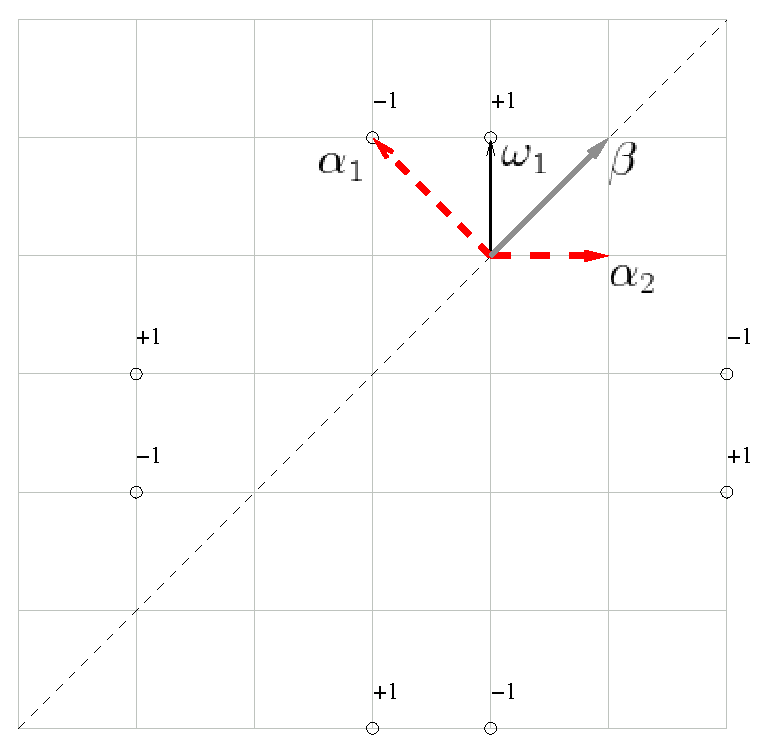
\includegraphics[width=60mm]{figures/figure1}
      \hfill
      \caption{Roots of $B_{2},A_{1}$ and $\Psi ^{\omega_1  }$}
      \hfill
      \vspace{5mm}
      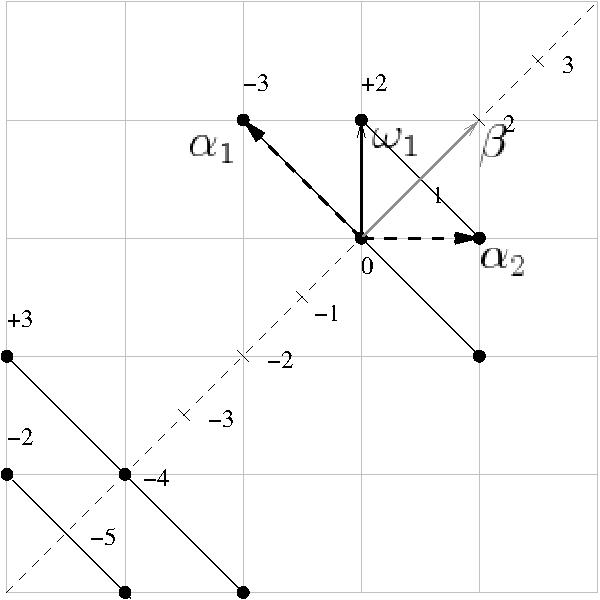
\includegraphics[width=60mm]{figures/figure2}
      \caption{Orthogonal subalgebra $\mathfrak{b}$ and dimensions of  $\mathfrak{b}$-modules}
    \end{multicols}
  \end{figure}
\end{frame}
\subsection{Affine example}
\begin{frame}
  \begin{figure}[t]
    \vspace*{-0.5cm}
    \begin{multicols}{2}
      \hfill
      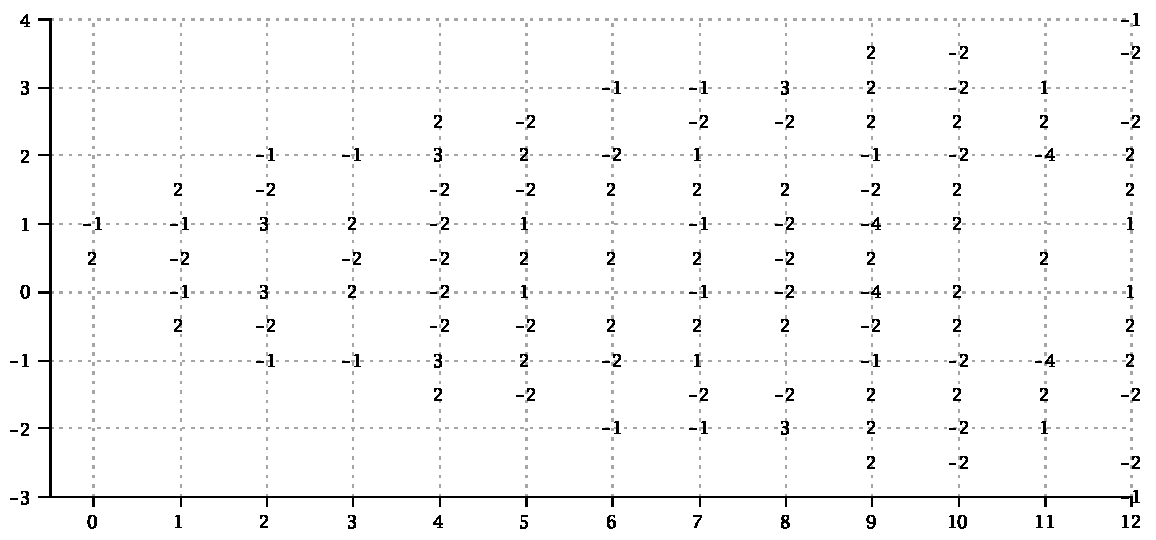
\includegraphics[width=60mm]{figures/figure10}
      \hfill
      \caption{$\Gamma_{\hat A_1\subset \hat B_2}$}
      \hfill
      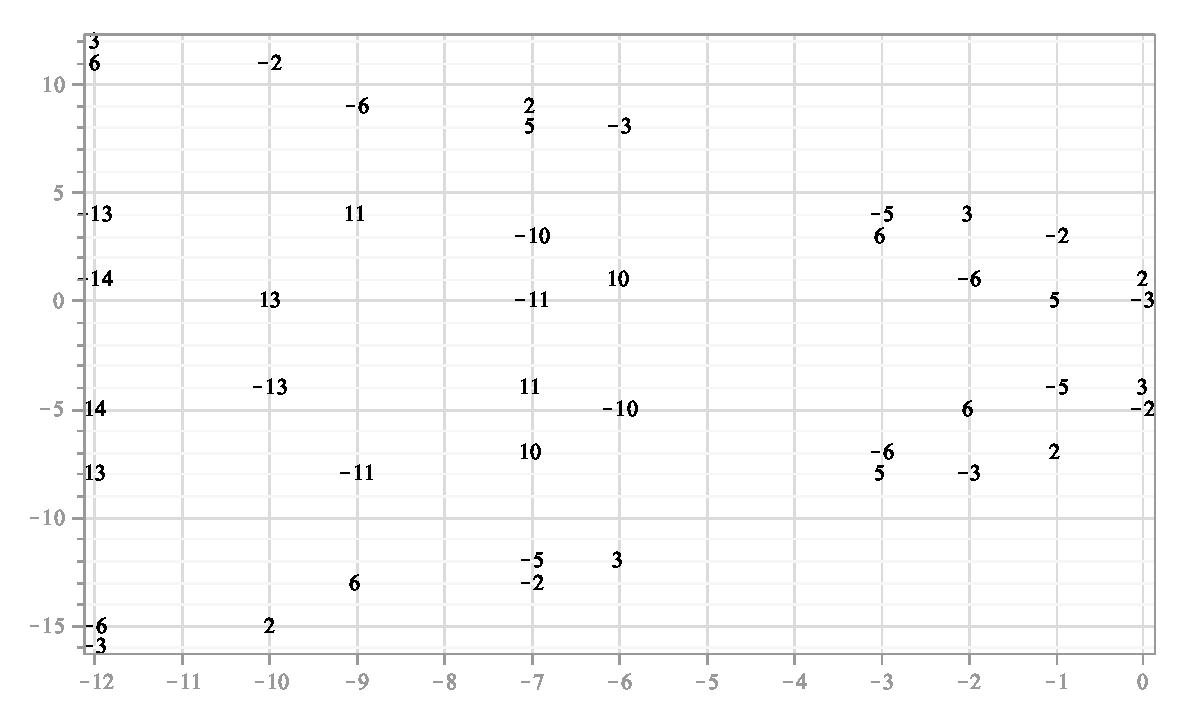
\includegraphics[width=60mm]{figures/figure12}
      \caption{ $\pi_{\hat A_{1}}\left( \Psi ^{\omega_1  }_{\hat B_{2}}\right)$}
    \end{multicols}
  \end{figure}
  \begin{figure}[b]
    \vspace*{-1.3cm}
    \centering
      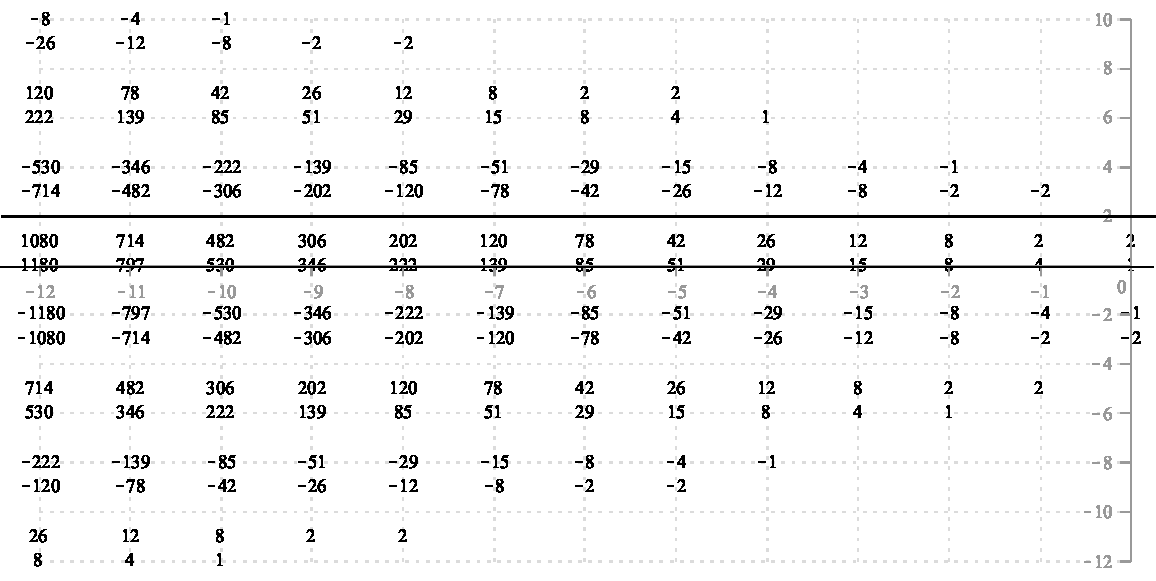
\includegraphics[width=100mm]{figures/figure13}
    \caption{Signed branching coefficients for $\hat A_1\subset \hat B_2$}
    \label{fig:2}
  \end{figure}
\end{frame}

\section{Splints and embeddings}
\begin{frame}
  \frametitle{Splints}
  \begin{Def}
$\phi $ -- ``embedding'' $\Delta_{0}\hookrightarrow \Delta$:
$\phi (\gamma )=\phi (\alpha )+\phi (\beta )\quad  \forall \alpha ,\beta ,\gamma \in P_{0}: \gamma =\alpha+\beta.$

\end{Def}
$\phi$ induces embedding of formal algebras: ${\mathcal{E}}_0\hookrightarrow \mathcal{E}$ and for ${\mathcal{E}}_i=\mathrm{Im}_{\phi}\left( {\mathcal{E}}_0\right)$ and $\phi^{-1}:{\mathcal{E}}_i \longrightarrow {\mathcal{E}}_0$.

\begin{Def}
Root system $\Delta$ ``splints'' to  $(\Delta _{1},\Delta _{2})$ if there exist embeddings  $\phi _{1}:\Delta _{1}\hookrightarrow \Delta $ and $\phi _{2}:\Delta _{2}\hookrightarrow \Delta $ where (a) $\Delta $ -- disjoint union of images of $\phi _{1}$ and $\phi _{2}$, (b) rank of  $\Delta _{1}$ and rank  $\Delta _{2}$ is less or equal to rank of $\Delta $.
\end{Def}
Let $\Delta _{1}=\Delta _{\af}$. $\Delta _{\sfr}:=\Delta_{2}=\Delta \setminus \Delta _{\af}$ determines injection fan  $\Gamma _{\af\hookrightarrow \gf}$. 
$\prod_{\beta \in \Delta _{\sfr}^{+}}\left( 1-e^{-\beta }\right)
=-\sum_{\gamma \in P}s(\gamma )e^{-\gamma }$

$\Psi _{\gf}^{\left( \mu \right) }=e^{-\rho}\sum_{w\in W_{\af}}w\circ \left(
e^{\rho _{\af}}\phi_{2}\left(\Psi ^{\widetilde{\mu }+\rho _{\sfr}}\right)\right) \quad \mu=\sum m_{k}\omega ^{k},\;\widetilde{\mu }=\sum m_{k}\omega _{\sfr}^{k}$

\end{frame}
\begin{frame}
  \frametitle{Example}
  \vspace{-0.5cm}
\begin{figure}[h!bt]
  \hspace*{-1.2cm}

   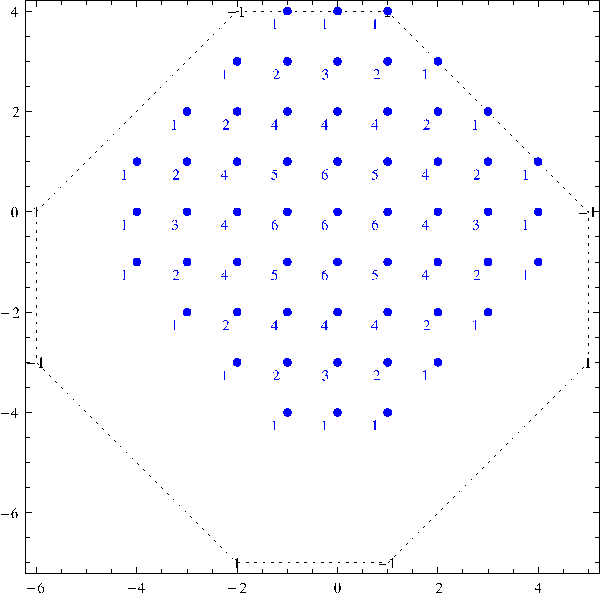
\includegraphics[width=50mm]{figures/b2}
   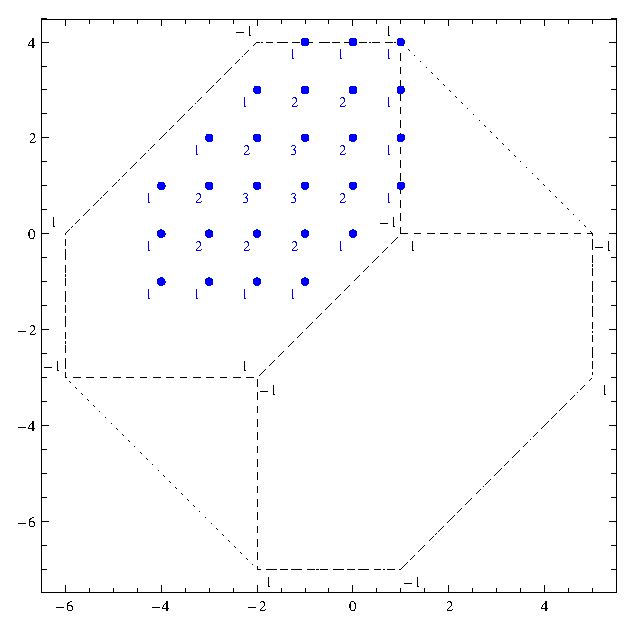
\includegraphics[width=50mm]{figures/b2-a2-a1}
  \caption{Weights and multiplicities of  $L^{[3,2]}_{B_{2}}$ on the left. Short dash is a singular element contour. On the right is a decomposition of singular element $\Psi_{B_{2}}(L^{[3,2]}_{B_{2}})$ into sum of images of singular elements $\Psi_{A_{2}}(L^{[3,2]})$ (long dash).  $L^{[3,2]}_{A_{2}}$ multiplicities =  branching coefficients for  $L^{[3,2]}_{B_{2}\downarrow A_{1}\oplus u(1)}$.}

 \label{fig:b2_splint}
\end{figure}

\end{frame}

\subsection{$G_2$}
\begin{frame}
  
  \begin{figure}[h!bt]
  \noindent\centering{
   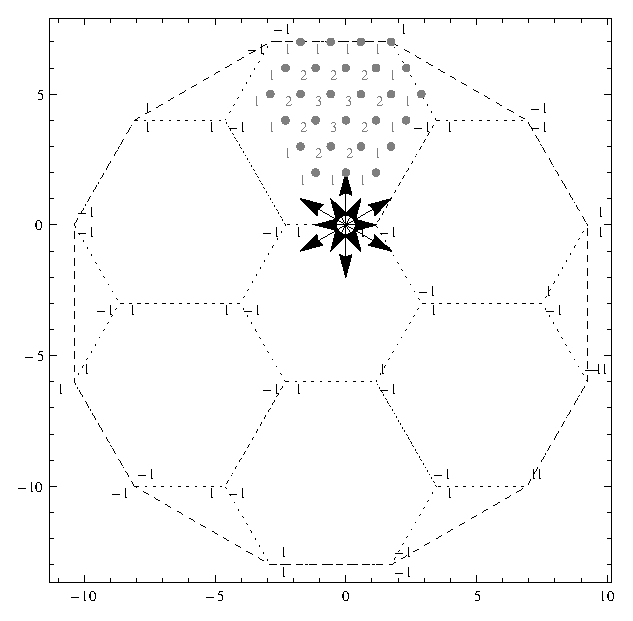
\includegraphics[width=65mm]{figures/g2}
  }

  \caption{Weyl group orbit  (long dash) for  $\Psi_{G_{2}}(L^{[3,2]})$ and its decomposition into sum of images of singular elements of   $A_{2}$ modules (short dash). Weight multiplicities of  $L^{[3,2]}_{A_{2}}$ coincide with branching coefficients $L^{[3,2]}_{G_{2}\downarrow A_{2}}$.}


 \label{fig:g2_splint}
\end{figure}

\end{frame}

\subsection{Affine Lie algebras}
\begin{frame}
Affine extension $\afh\subset\gfh$. Since $\mathrm{rank}\gf\leq\mathrm{rank} \af+\mathrm{rank}\sfr$ for Weyl denominators we have 
\begin{multline*}
\prod_{\alpha\in\hat{\Delta}^{+}_{1}}(1-e^{-\alpha})^{\mathrm{mult}(\alpha)}\prod_{\beta\in\hat{\Delta}^{+}_{2}}(1-e^{\phi\circ \beta})^{\mathrm{mult}(\beta)}=\\
\prod_{\gamma\in\hat{\Delta}^{+}}(1-e^{-\gamma})^{\mathrm{mult}(\gamma)}\prod_{n=0}^{\infty}(1-e^{-n\delta})^{\mathrm{rank}\af+\mathrm{rank}\sfr-\mathrm{rank}\gf}
\end{multline*}
 $$\Theta^{(\gfh)}_{\widehat{\lambda}=(\lambda,k,0)}(\tau,z)=\sum_{\xi\in Q_{\gf}+\frac{\lambda}{k}}e^{2\pi i k \left(\frac{1}{2} (\xi,\xi) \tau + (\xi,z)\right)}$$
Then we obtain relation on theta-functions of algebras $\gfh,\hat\sfr,\afh$:
\begin{multline*}
  \left(\sum_{v\in W_{\af}}\epsilon(v) \Theta^{(\afh)}_{v\rho_{\af}}(\tau,z)\right)
  \cdot \left(\sum_{u\in W_{\sfr}}\epsilon(u) \Theta^{(\hat{\sfr})}_{\phi\circ(u\rho_{\sfr})}(\tau,z)\right)= \\
  \left(\sum_{w\in W}\epsilon(w) \Theta^{(\gfh)}_{w\rho_{\gf}}(\tau,z)\right)
\end{multline*}
\end{frame}
\begin{frame}
  \frametitle{Branching to finite-dimensional subalgebras}

Consider branching of  $\gfh$-module to  $\gf$-modules
\begin{equation*}
  \label{eq:149}
\mathrm{ch}L^{\hat{\mu}}_{\gfh}=\sum_{n=0}^{\infty}e^{-n\delta} \sum_{\nu\in P} b^{(\hat{\mu})}_{\nu}(n) \mathrm{ch} L^{\nu}_{\gf} \quad m^{(\hat{\mu})}_{\hat{\nu}=(\nu,k,n)}=\sum_{\xi\in P}
b^{(\hat{\mu})}_{\xi}(n) m^{(\xi)}_{\nu}
\end{equation*}
Introduce functions $b^{(\hat{\mu})}_{\nu}(q):=\sum_{n=0}^{\infty} b^{(\hat{\mu})}_{\nu}(n) q^{n}$, which are connected with  $q$-dimension \\ $\mathrm{dim}_{q}L^{\hat \mu}_{\gfh}=\sum_{n=0}^{\infty}q^{n}\sum_{\nu\in P} b^{(\hat \mu)}_{\nu}(n) \mathrm{dim }L^{\nu}_{\gf}=\sum_{\nu\in P}b^{(\hat\mu)}_{\nu}(q) \mathrm{dim} L^{\nu}_{\gf}$.

 $ \sigma^{(\hat{\mu})}_{\nu}(q) = \sum_{\xi\in P} m^{(\xi)}_{\nu} b^{(\hat{\mu})}_{\xi}(q)$.

Introduce the order on the set of the roots $\xi$:
assign to the weight   $\xi$ the value  $(\rho,\xi)$ and order weights using this values. Then  $$\sigma(q)=M b(q)\quad b(q)=M^{-1}\sigma(q)$$
  $\sigma(q)$ and  $b(q)$ are infinite vectors of string functions and branching functions. The matrix $M$ contains weight multiplicities of  $\gf$-modules. Inverse matrix $M^{-1}$ consists of recurrent relations on weight multiplicities.
\end{frame}
\begin{frame}
    \frametitle{Matrix relations for splints}
Consider branching of  $\gfh$-modules into  $\af$-modules when there exists a splint
$\Delta^{+}_{\gf}=\Delta^{+}_{\af}\cup \phi(\Delta^{+}_{\sfr})$.
Decompose  $\gf$-modules into 
$\af$-modules using splint properties:
\begin{multline}
  \label{eq:125}
  \mathrm{ch}L^{\hat{\mu}}_{\gfh}=
\sum_{n=0}^{\infty}e^{-n\delta} \sum_{\nu\in P_{\af}} b^{(\hat{\mu})}_{(\gfh\downarrow\af)\nu}(n) \mathrm{ch} L^{\nu}_{\af}=\\
\sum_{n=0}^{\infty} e^{-n\delta} \sum_{\nu\in P} b^{(\hat{\mu})}_{(\gfh\downarrow\gf )\nu}(n) \sum_{\xi\in P_{\af}} b^{(\nu)}_{(\gf\downarrow \af) \xi}\mathrm{ch} L^{\xi}_{\af}=\\
=\sum_{n=0}^{\infty} e^{-n\delta} \sum_{\nu\in P} b^{(\hat{\mu})}_{(\gfh\downarrow\gf )\nu}(n) \sum_{\xi\in P_{\af}} M^{\widetilde{\nu}}_{  \widetilde{\nu}-\phi^{-1}( \nu-\xi )}\mathrm{ch} L^{\xi}_{\af}
\end{multline}
Matrix relation holds for branching functions $b_{(\gfh\downarrow\af)}(q)= M_{\sfr}\;
b_{(\gfh\downarrow\gf)}(q)$ and
$\sigma(q)=M_{\af}\; b_{(\gfh\downarrow\af)}(q)$.  If we know branching coefficients for the embedding $\gf\subset\gfh$ we immediately obtain (graded) branching functions for the embedding $\af\subset \gfh$.
\end{frame}


\section{Conclusion}


\begin{frame}
  \frametitle{Conclusion}
  \begin{itemize}
  \item Singular elements determine structure of modules
  \item Decomposition of singular element leads to relations on branching coefficients
  \item We can get different decompositions and new relations if we consider deformed root subsystems
  \end{itemize}
\end{frame}
\begin{frame}
  \frametitle{Thank you!}
\end{frame}

\end{document}
